\chapter{閉じた弦、レベルマッチング、双対性}

\lectureoverview{閉じた弦は、その二つの内在的な方向に独立な波を支える。それらの波を量子化すると、一見したところ開いた弦の光子が二重になるように思われるが、弦座標の原点をずらす変換の下での不変性が、片側だけの状態を取り除く。生き残る最初のレベルには、質量ゼロのスピン2の粒子が含まれる。記述を変えるという同じ考え方は、さらに広い問いを開く。結合定数が変化するとき、ある対象が基本的であるとはどういうことか。}

\section{温存された生成子}

閉じた弦を描く前に、正準力学から一つの事実を思い出しておこう。
\begin{equation}
  L=L(q_i,\dot q_i),
\end{equation}
とし、\(q_i\)に共役な運動量を
\begin{equation}
  p_i=\frac{\partial L}{\partial\dot q_i}.
\end{equation}
で定義する。無限小の連続変換は
\begin{equation}
  \delta q_i=\epsilon f_i(q),
  \label{eq:l04-infinitesimal-transformation}
\end{equation}
と書ける。ここで\(\epsilon\)は小さなパラメータである。この変換が対称性であれば、ネーターの定理が保存電荷を与える。座標の変位を共通のパラメータで割ると、生成子
\begin{equation}
  Q=\sum_i p_i f_i(q)
   =\frac{1}{\epsilon}\sum_i p_i\,\delta q_i.
  \label{eq:l04-noether-charge}
\end{equation}
が得られる。量子力学では、\(Q\)は対応する小さな変換を生成する演算子である。

\(xy\)平面内の回転がよく知られた例である。向きの一つの選び方では
\begin{equation}
  \delta x=\epsilon y,
  \qquad
  \delta y=-\epsilon x,
\end{equation}
であり、\eqref{eq:l04-noether-charge}は同じ符号の選び方の下で角運動量になる。この特定の例は問題ではない。重要なのはパターンである。運動量を無限小変位と縮約すると生成子が得られる。

\begin{figure}[H]
  \centering
  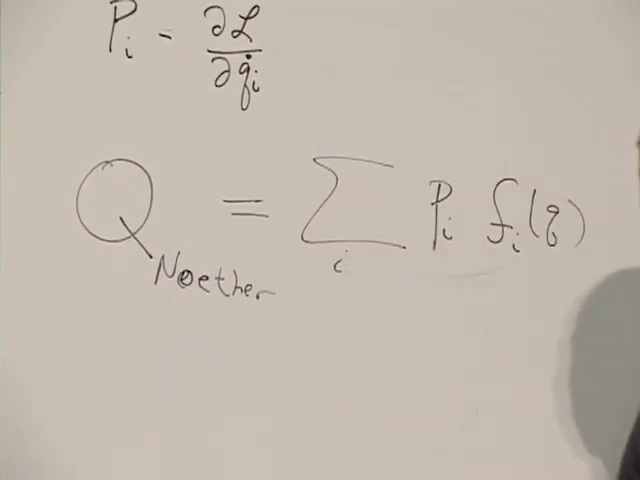
\includegraphics[width=0.76\textwidth]{lecture_04_figure_01.png}
  \caption{閉じた弦の座標の後でのずらしのために温存された正準運動量とネーター生成子。}
  \lectureframe{00:05:00}
  \label{fig:l04-noether-board}
\end{figure}

まもなく、その座標が通常の空間内の点ではなく、弦に沿った点のラベル付けであるような対称性に出会う。式\eqref{eq:l04-noether-charge}はその目的のために手の届くところに置かれている。

\section{ループに沿った座標}

閉じた弦には端点がない。パラメータ
\begin{equation}
  0\leq \sigma<2\pi
\end{equation}
を選び、当面は一つの点を\(\sigma=0\)と印づける。半周した点は\(\sigma=\pi\)であり、四分の一回転と四分の三回転は\(\pi/2\)と\(3\pi/2\)である。この印は座標の規約を定めるものであり、まだ物理的な特徴ではない。

\begin{figure}[H]
  \centering
  \begin{minipage}[t]{0.58\textwidth}
    \centering
    \includegraphics[width=\textwidth]{lecture_04_figure_02.png}
    \par\smallskip\footnotesize (a) 黒板上の印をつけたループ。
  \end{minipage}\hfill
  \begin{minipage}[t]{0.37\textwidth}
    \centering
    \begin{adjustbox}{max width=\linewidth}
    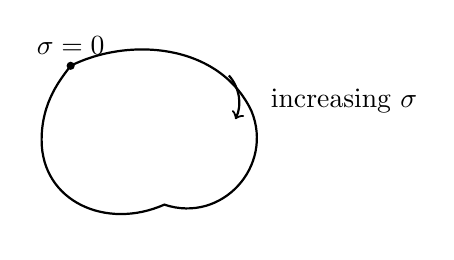
\begin{tikzpicture}[scale=0.82]
      \draw[thick]
        (0.1,1.1)
        .. controls (1.0,1.55) and (2.4,1.45) .. (2.9,0.4)
        .. controls (3.25,-0.45) and (2.45,-1.35) .. (1.55,-1.05)
        .. controls (0.65,-1.45) and (-0.35,-1.0) .. (-0.35,-0.05)
        .. controls (-0.35,0.55) and (-0.05,0.9) .. (0.1,1.1);
      \fill (0.1,1.1) circle (1.8pt);
      \node[above] at (0.1,1.12) {\(\sigma=0\)};
      \draw[->,thick] (2.55,0.95) arc[start angle=42,end angle=-25,radius=0.62];
      \node[right] at (3.05,0.55) {increasing \(\sigma\)};
    \end{tikzpicture}
    \end{adjustbox}
    \par\smallskip\footnotesize (b) 内在的な向き。
  \end{minipage}
  \caption{原点を定めるために一点が印づけられ、矢印が\(\sigma\)が増加する向きを固定する。}
  \lectureframe{00:06:48}
  \label{fig:l04-closed-string-origin}
\end{figure}

ループに沿った矢印は\emph{内在的な}向きである。これは\(xy\)平面内の時計回りや反時計回りの運動と混同してはならない。印をつけた輪ゴムが板から持ち上げられ、裏返され、元に戻されるのを想像しよう。その見かけの時計回りの向きは逆になるが、内在的な印の順序は変わらない。\(\sigma\)が増加することは\(\sigma\)が増加することのままである。

この区別が右向き波と左向き波の言葉遣いを支配する。この章では、右向きの擾乱とは\(\sigma\)が増加する向きに進むものを意味し、左向きの擾乱とは\(\sigma\)が減少する向きに進むものを意味する。どちらの名前も、その擾乱が部屋の中でどちらに動いて見えるかは教えてくれない。

向きは元々のハドロン弦の描像において具体的な役割を持っていた。向きづけられたフラックスチューブを切ると、一方の端点にクォーク、他方の端点に反クォークが生じる。内在的な矢印が二つの端を区別する。向きづけられていない弦理論を構成することもできるが、当面の議論では矢印とそれに沿った二つの向きを保つ。

\section{周期性と進行波}

\(X(\sigma,\tau)\)と\(Y(\sigma,\tau)\)を弦の二つの横座標とし、\(\tau\)は時間を表すものとする。余分な横座標が存在する場合には、まったく同じように扱われる。\(\sigma=0\)と\(\sigma=2\pi\)は同じ点をラベルするので、
\begin{equation}
  X(\sigma+2\pi,\tau)=X(\sigma,\tau),
  \qquad
  Y(\sigma+2\pi,\tau)=Y(\sigma,\tau).
  \label{eq:l04-periodicity}
\end{equation}

\begin{figure}[H]
  \centering
  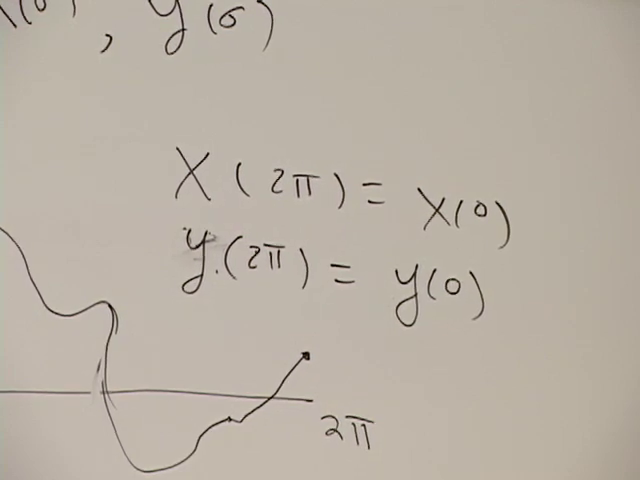
\includegraphics[width=0.76\textwidth]{lecture_04_figure_03.png}
  \caption{二つの横座標に対する周期的境界条件。}
  \lectureframe{00:12:40}
  \label{fig:l04-periodicity-board}
\end{figure}

したがって、局在した揺れは無限に循環することができる。それが\(2\pi\)に達すると、単に\(0\)に再び現れる。これは開いた弦とは異なる。開いた弦では、進行波は端点に達して反射し、左向きであったものが右向きになり、その逆も同様である。定在波は開いた弦にとって自然であるのに対し、閉じた弦は独立に伝播する二つの族を許す。

\subsection{複素フーリエモード}

周期関数にとって便利な基底は
\begin{equation}
  e^{in\sigma}=\cos(n\sigma)+i\sin(n\sigma),
  \qquad n\in\mathbb Z.
\end{equation}
である。整数条件は周期性によって強制される：
\(e^{in(\sigma+2\pi)}=e^{in\sigma}\)。例えば\(n\)を半整数に置き換えると、一周した後で関数が変わってしまう。

時間依存性を一時的に抑えて書くと、黒板での展開は
\begin{align}
  X(\sigma)
  &=
  X_0+
  \sum_{n>0}X_n e^{in\sigma}
  +\sum_{n>0}X_{-n}e^{-in\sigma},
  \label{eq:l04-fourier-x}\\
  Y(\sigma)
  &=
  Y_0+
  \sum_{n>0}Y_n e^{in\sigma}
  +\sum_{n>0}Y_{-n}e^{-in\sigma}.
  \label{eq:l04-fourier-y}
\end{align}
である。実数\(X\)と\(Y\)に対して、古典的レベルでは負の指数の係数は正の指数の係数の複素共役である。ゼロモード\(X_0\)と\(Y_0\)は重心の位置を与える。それらは位置であり、内部振動ではない。

\begin{figure}[H]
  \centering
  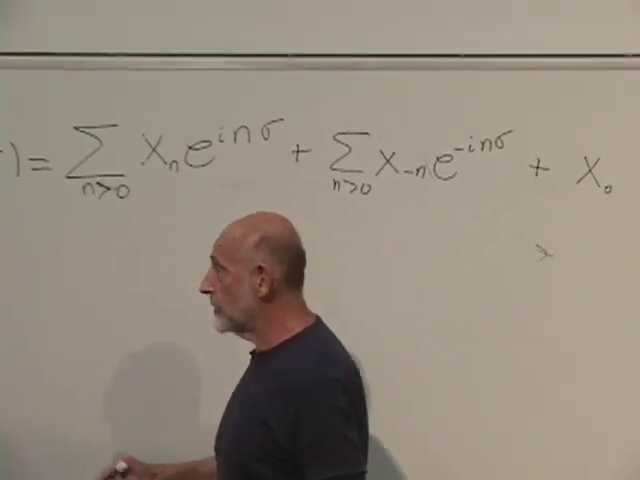
\includegraphics[width=0.82\textwidth]{lecture_04_figure_04.png}
  \caption{周期フーリエ展開の正および負の指数の部分、続いてゼロモード。}
  \lectureframe{00:20:00}
  \label{fig:l04-fourier-board}
\end{figure}

\begin{classroomqa}
\audiencequestion{これらが進行する波であるなら、時間座標はどこにあるのか。\lecturetimestamp{00:19:05}}
\lecturerresponse{黒板の記法ではそれが抑えられているだけである。進行解は\(\sigma\)と\(\tau\)の両方を含む位相を担う。以下で用いる規約では、一方の族は
\(e^{-in(\tau-\sigma)}\)
をもち、他方の族は
\(e^{-in(\tau+\sigma)}\)
をもつ。}
\end{classroomqa}

したがって、伝播を決めるのは、純粋に空間的なフーリエ因子における\(n\)の符号そのものではなく、完全な位相である。次のように書ける：
\begin{equation}
  X(\sigma,\tau)=X_R(\tau-\sigma)+X_L(\tau+\sigma),
  \label{eq:l04-chiral-solution}
\end{equation}
また\(Y\)についても同様である。どちらの族を\(L\)ではなく\(R\)と呼ぶかは規約である。不変な事実は、\(\sigma\)円に沿って二つの反対向きの方向が存在することである。\editorialnote{ある瞬間における因子\(e^{in\sigma}\)は、それだけでは進行する波を指定しない。伝播は時間位相が与えられて初めて確定する。}

\section{二つの方向のエネルギー}

局所的な力学は開いた弦の場合と同じである。ここで用いる簡略化された規格化では、
\begin{equation}
  L\propto
  \int_0^{2\pi}d\sigma\,
  \left[
    \dot X^2-X'^2+\dot Y^2-Y'^2
  \right],
  \label{eq:l04-string-lagrangian}
\end{equation}
ここでドットは\(\partial_\tau\)を表し、プライムは
\(\partial_\sigma\)を表す。エネルギーでは運動項と弾性項の間にプラス符号がつく：
\begin{equation}
  E\propto
  \int_0^{2\pi}d\sigma\,
  \left[
    \dot X^2+X'^2+\dot Y^2+Y'^2
  \right].
  \label{eq:l04-string-energy}
\end{equation}
どちらの横座標についても、
\begin{equation}
  \dot X^2+X'^2
  =
  \frac12(\dot X+X')^2+
  \frac12(\dot X-X')^2.
  \label{eq:l04-energy-square-completion}
\end{equation}
交差項は相殺し、ちょうど元の運動エネルギーと勾配エネルギーが残る。

\begin{figure}[H]
  \centering
  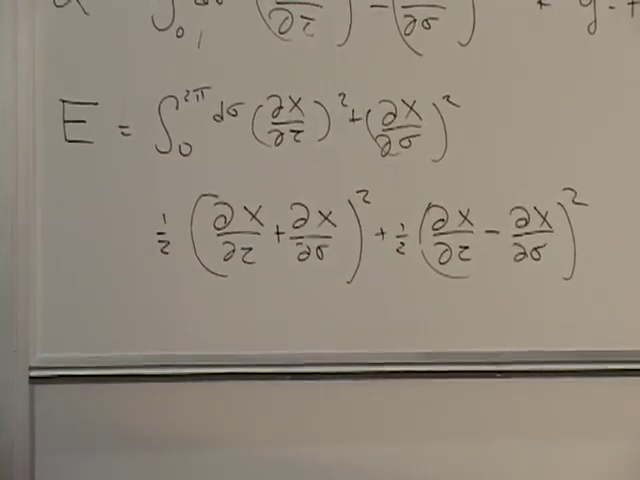
\includegraphics[width=0.82\textwidth]{lecture_04_figure_05.png}
  \caption{全エネルギーを二つの進行波のセクターに再編成したもの。}
  \lectureframe{00:25:10}
  \label{fig:l04-energy-board}
\end{figure}

\(X_R(\tau-\sigma)\)に対しては\(\dot X_R=-X_R'\)が成り立ち、
\(X_L(\tau+\sigma)\)に対しては\(\dot X_L=X_L'\)が成り立つ。したがって\eqref{eq:l04-energy-square-completion}における二つの平方は、二つのカイラルな族を分離する。すべての横座標を含めて、
\begin{align}
  E_L&\propto
  \frac12\int_0^{2\pi}d\sigma
  \sum_I(\dot X^I+X^{I\prime})^2,\\
  E_R&\propto
  \frac12\int_0^{2\pi}d\sigma
  \sum_I(\dot X^I-X^{I\prime})^2.
  \label{eq:l04-left-right-energies}
\end{align}
と定義する。このとき\(E=E_L+E_R\)である。この段階では方程式が線形であるため、二つのセクターからの波は散乱せずに互いを通り抜ける。

\subsection{二倍の数の振動子}

フーリエ級数を
\eqref{eq:l04-string-lagrangian}
に代入すると、各非ゼロモード係数は調和振動子になる。その振動数は\(|n|\)に比例する。より短い波長はより高い振動数を意味し、したがってより大きな励起エネルギーを意味する。開いた弦とは異なり、各正の振動数は独立に伝播する二つのコピーに現れる。

黒板では\(X\)偏極の生成演算子を\(a_n^+\)および\(a_{-n}^+\)と書き、\(Y\)偏極のものを
\(b_n^+\)および\(b_{-n}^+\)と書いている。生成と伝播をより明確に分離するために、次のように書くことにする：
\begin{equation}
  a_n^\dagger,\quad b_n^\dagger,
  \qquad
  \widetilde a_n^\dagger,\quad\widetilde b_n^\dagger,
  \qquad n>0.
  \label{eq:l04-oscillator-notation}
\end{equation}
チルダのない演算子とチルダ付きの演算子は、世界面の反対向きの方向を生成する。\(a\)と\(b\)は二つの横偏極を表す。

\begin{figure}[H]
  \centering
  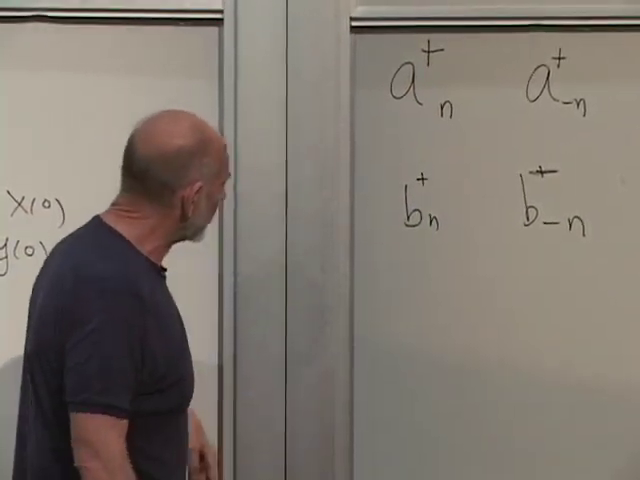
\includegraphics[width=0.65\textwidth]{lecture_04_figure_06.png}
  \caption{二重化された\(X\)偏極および\(Y\)偏極の生成演算子に対する黒板の記法。}
  \lectureframe{00:29:10}
  \label{fig:l04-oscillators-board}
\end{figure}

\(N_n^{(a)},N_n^{(b)}\)およびそのチルダ付きの相棒が占有数であるなら、二つの方向に担われる振動子準位は概略的に
\begin{equation}
  \begin{aligned}
    N&=\sum_{n>0}n\bigl(N_n^{(a)}+N_n^{(b)}+\cdots\bigr),\\
    \widetilde N&=\sum_{n>0}n
      \bigl(\widetilde N_n^{(a)}+\widetilde N_n^{(b)}+\cdots\bigr).
  \end{aligned}
  \label{eq:l04-level-operators}
\end{equation}
である。省略記号は追加の横方向を表す。

\section{失敗するスペクトルの推測}

開いた弦の第一準位を思い出そう。基底状態に\(a_1^\dagger\)または\(b_1^\dagger\)を作用させると二つの線形偏極が得られる。それらの円偏極の組み合わせ
\begin{equation}
  c_\pm^\dagger
  =
  \frac{1}{\sqrt2}
  \left(a_1^\dagger\pm i b_1^\dagger\right),
  \label{eq:l04-open-circular}
\end{equation}
はヘリシティ\(h=\pm1\)を担う。ヘリシティゼロの相棒が存在しないことが、この初等的な四次元記述における質量ゼロベクトルの特徴である。

閉じた弦の基底状態の質量二乗を\(m_0^2\)とする。まず素朴な推測は、
\begin{equation}
  a_1^\dagger,\quad b_1^\dagger,\quad
  \widetilde a_1^\dagger,\quad\widetilde b_1^\dagger.
  \label{eq:l04-naive-one-sided}
\end{equation}
のいずれか一つを一度作用させるというものである。これは開いた弦の光子の二つのコピー、すなわち各伝播方向に一つずつを思わせる。しかし次のエネルギーでは、制限のないリストは妥当な回転多重項にまとまらない。問題はより込み入った記帳によっても修復されない。すべての振動子単項式が物理的状態であるという前提が誤っているのである。

\subsection{まず規則としてのレベル整合}

物理的な閉じた弦の条件は
\begin{equation}
  N=\widetilde N,
  \qquad\text{equivalently}\qquad E_L=E_R.
  \label{eq:l04-level-matching}
\end{equation}
である。今のところこれを公準として受け取り、その起源はそれが何を達成するかを見た後に初めて導出する。

\eqref{eq:l04-naive-one-sided} のすべての状態は、一方のセクターに1単位のエネルギーを持ち、他方には持たないので、すべて除外される。最初に生き残る状態は、各ファミリーから1個ずつの振動子を運ぶ：
\begin{align}
  a_1^\dagger\widetilde a_1^\dagger\ket{0},
  &\qquad
  b_1^\dagger\widetilde b_1^\dagger\ket{0},
  \label{eq:l04-four-matched-a}\\
  a_1^\dagger\widetilde b_1^\dagger\ket{0},
  &\qquad
  b_1^\dagger\widetilde a_1^\dagger\ket{0}.
  \label{eq:l04-four-matched-b}
\end{align}
これらは全振動子エネルギー2を持ち、二つの方向に等しく分配されている。単一の \(n=2\) 生成演算子も同じ全振動子エネルギーを持つが、\eqref{eq:l04-level-matching} を満たさない；それは片側だけに2単位を寄与する。

\begin{figure}[H]
  \centering
  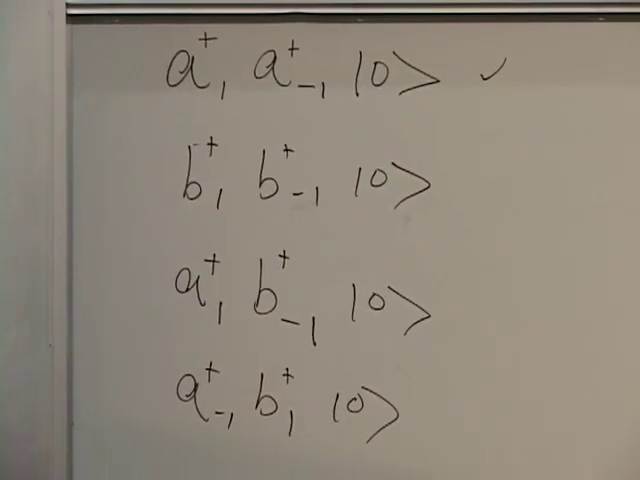
\includegraphics[width=0.70\textwidth]{lecture_04_figure_07.png}
  \caption{レベルマッチングを生き残る4つの第1レベル状態。ボードでは下付き文字\(1\)と\(-1\)を用いているが、\eqref{eq:l04-four-matched-a}--\eqref{eq:l04-four-matched-b}ではチルダなし演算子とチルダ付き演算子を用いている。}
  \lectureframe{00:41:05}
  \label{fig:l04-level-matched-board}
\end{figure}

\section{最初の整合レベルにおける重力子}

両方のカイラル・ファミリーを円基底に置く：
\begin{equation}
  c_\pm^\dagger
  =\frac{a_1^\dagger\pm i b_1^\dagger}{\sqrt2},
  \qquad
  \widetilde c_\pm^\dagger
  =\frac{\widetilde a_1^\dagger\pm i\widetilde b_1^\dagger}{\sqrt2}.
  \label{eq:l04-closed-circular}
\end{equation}
各因子は通常の横空間でヘリシティ \(+1\) または \(-1\) を寄与する。したがってそれらの積は次を与える：
\begin{center}
\begin{tabular}{c c}
  \toprule
  状態 & ヘリシティ \\
  \midrule
  \(c_+^\dagger\widetilde c_+^\dagger\ket0\) & \(+2\) \\
  \(c_-^\dagger\widetilde c_-^\dagger\ket0\) & \(-2\) \\
  \(c_+^\dagger\widetilde c_-^\dagger\ket0\) & \(0\) \\
  \(c_-^\dagger\widetilde c_+^\dagger\ket0\) & \(0\) \\
  \bottomrule
\end{tabular}
\end{center}

\begin{classroomqa}
\audiencequestion{第二の円偏光因子は反対の伝播セクターから来るべきか？\lecturetimestamp{00:43:20}}
\lecturerresponse{はい。ボードに最初に書かれた式は、まさにこの理由で訂正された。ここでの物理的状態は、一つの右移動振動子と一つの左移動振動子を対にしなければならない；そうでなければレベル整合しない。ヘリシティは横空間の偏光を指し、一方、二つの因子は反対の世界面方向を指す。}
\end{classroomqa}

\begin{figure}[H]
  \centering
  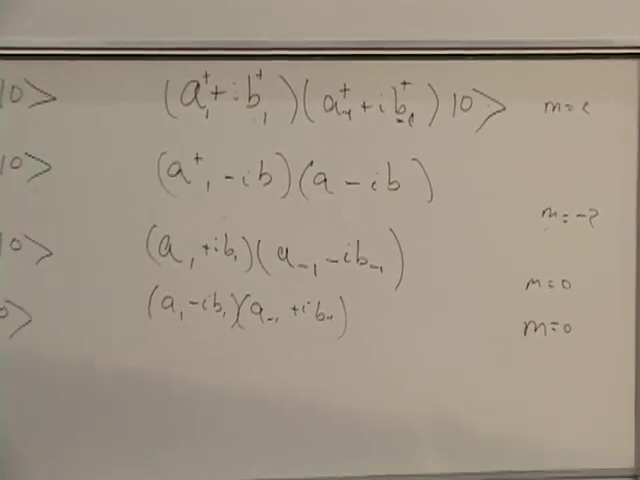
\includegraphics[width=0.82\textwidth]{lecture_04_figure_08.png}
  \caption{ボード訂正後の4つの円基底積。ヘリシティは \(+2,-2,0,0\)。}
  \lectureframe{00:46:10}
  \label{fig:l04-helicity-board}
\end{figure}

質量のあるスピン2粒子は5つのスピン射影を持つ：
\begin{equation}
  m=2,1,0,-1,-2.
\end{equation}
整合したレベルには \(m=\pm1\) パートナーが含まれない。したがってそれは質量のあるスピン2多重項ではありえない。対照的に、質量のないスピン2粒子はヘリシティ \(+2\) と \(-2\) のみを持つ。同じヘリシティの積はまさにそれら二つの状態である：それらは重力子偏光である。

ヘリシティゼロの組み合わせが二つ残る。授業で用いられた言葉では、一方はディラトンであり、他方はアクシオンである。一般的な閉じたボソン弦の共変的記述はこの主張を精密化する：
\begin{equation}
  \begin{aligned}
    \alpha_{-1}^{I}\widetilde\alpha_{-1}^{J}\ket{0;k}
    &\longrightarrow
    \underbrace{h_{IJ}}_{\text{symmetric traceless}}
    \oplus
    \underbrace{B_{IJ}}_{\text{antisymmetric}}\\
    &\hspace{2.5em}\oplus
    \underbrace{\Phi}_{\text{trace}}.
  \end{aligned}
  \label{eq:l04-massless-tensor-decomposition}
\end{equation}
これらは重力子、反対称2形式、およびディラトンである。4次元では2形式はアクシオン的擬スカラーに双対化でき、それが講義で採用された言葉である。\editorialnote{第二のヘリシティゼロ状態は、一般的な閉じた弦スペクトルにおける反対称テンソル場 \(B_{\mu\nu}\) である。それをアクシオンと呼ぶのは4次元双対記述である。}

この形式的なレベルでは、三つの場は質量がない。コンパクト化、射影、および背景力学は、どのスカラーまたは2形式自由度が軽いまま残るかを変えうる。重力子は異なる：ひとたび整合した相互作用する閉じた弦セクターが存在すれば、その質量のないスピン2状態は不可避である。これが、重力が別個の材料として付け加えられるのではなく、閉じた弦から現れる理由である。

\section{なぜレベルは整合しなければならないか}

ここで \(\sigma=0\) の印に戻る。それはループに付いた物理的なビーズなのか、それとも単に我々のパラメータの原点なのか？通常の印のない閉じた弦では、どの点も特権的であってはならない。量子状態は、すべてのラベルが一緒にずらされても変わらないままでなければならない。

\subsection{離散版}

ループを、横座標 \((X_i,Y_i)\) を持つ \(M\) 個の順序付けられた点として正則化する。一時的に \(Y_i\) を抑制する。配位空間波動関数は
\begin{equation}
  \Psi(X_1,X_2,\ldots,X_M).
\end{equation}
どの点を最初と呼ぶかを変えると巡回置換を与える：
\begin{align}
  \Psi(X_1,X_2,\ldots,X_M)
  &=
  \Psi(X_2,\ldots,X_M,X_1)\nonumber\\
  &=
  \Psi(X_3,\ldots,X_M,X_1,X_2).
  \label{eq:l04-cyclic-wavefunction}
\end{align}
これは任意の置換の下での不変性ではない。たとえば \(X_1\) と \(X_2\) の間に \(X_3\) を挿入すると、隣接構造が変わり、離散化された弦を実質的に引き裂いて再接続する。共通の巡回的再ラベリング
\begin{equation}
  X_i\longrightarrow X_{i+1}\qquad(\text{mod }M)
  \label{eq:l04-discrete-shift}
\end{equation}
のみが、好まれる原点の不在を表す。

\begin{figure}[H]
  \centering
  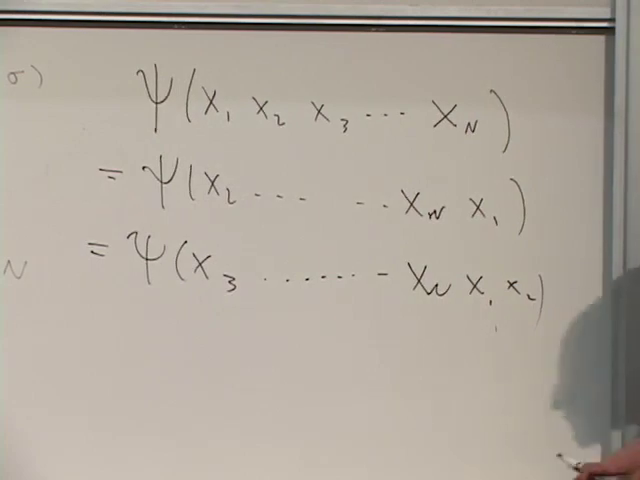
\includegraphics[width=0.82\textwidth]{lecture_04_figure_09.png}
  \caption{離散化された閉じた弦に対する巡回波動関数の恒等式。}
  \lectureframe{00:56:20}
  \label{fig:l04-cyclic-board}
\end{figure}

\subsection{連続版}

連続極限 \(M\to\infty\) では、状態は波動汎関数
\begin{equation*}
  \Psi[X(\sigma),Y(\sigma)].
\end{equation*}
巡回的再ラベリングは次になる：
\begin{equation}
  \sigma\longrightarrow\sigma+\epsilon.
\end{equation}
不変性は次を言う：
\begin{equation}
  \Psi[X(\sigma+\epsilon),Y(\sigma+\epsilon)]
  =
  \Psi[X(\sigma),Y(\sigma)].
  \label{eq:l04-wavefunctional-invariance}
\end{equation}

\begin{figure}[H]
  \centering
  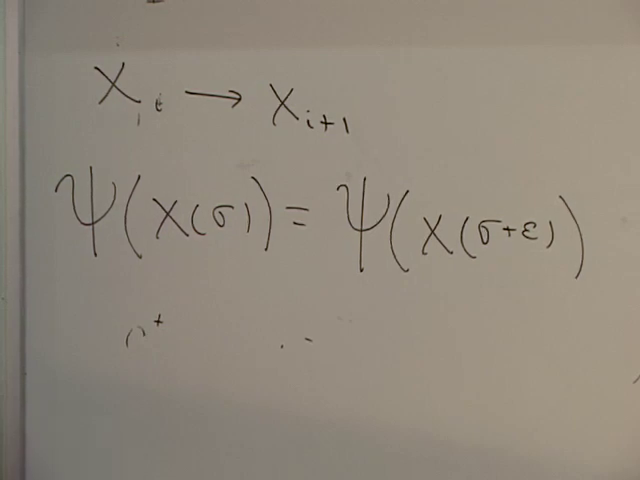
\includegraphics[width=0.72\textwidth]{lecture_04_figure_10.png}
  \caption{離散シフトとその波動汎関数連続形。}
  \lectureframe{00:58:40}
  \label{fig:l04-wavefunctional-board}
\end{figure}

一次のオーダーでは、
\begin{equation}
  \delta X(\sigma)=\epsilon X'(\sigma),
  \qquad
  \delta Y(\sigma)=\epsilon Y'(\sigma),
  \label{eq:l04-profile-shift}
\end{equation}
ただし、プロファイルの能動的シフトと座標の受動的シフトを区別する全体符号までは除く。対応する波動汎関数の変分は
\begin{equation}
  \delta\Psi
  =
  \epsilon\int_0^{2\pi}d\sigma
  \left[
    \frac{\delta\Psi}{\delta X(\sigma)}X'(\sigma)
    +
    \frac{\delta\Psi}{\delta Y(\sigma)}Y'(\sigma)
  \right].
  \label{eq:l04-functional-variation}
\end{equation}

\begin{figure}[H]
  \centering
  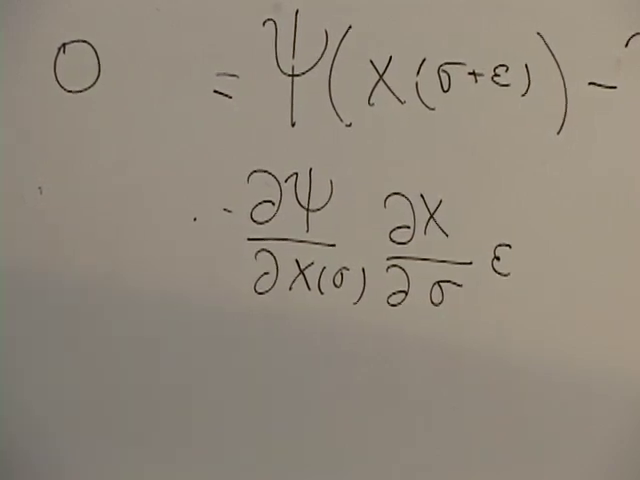
\includegraphics[width=0.72\textwidth]{lecture_04_figure_11.png}
  \caption{シフトされた波動汎関数の引数の一次展開。}
  \lectureframe{01:01:31}
  \label{fig:l04-functional-expansion-board}
\end{figure}

\begin{classroomqa}
\audiencequestion{一次の条件は\(\sigma\)の各値に対する別々の方程式か？\lecturetimestamp{01:01:30}}
\lecturerresponse{いいえ。変換は弦のすべての点を一緒にシフトする。ある点での変分は他のすべての点での変分に加えられなければならず、そのため連続体の表式には\(\sigma\)にわたる積分が含まれる。}
\end{classroomqa}

座標表示では、
\begin{equation}
  P_X(\sigma)=-i\frac{\delta}{\delta X(\sigma)},
  \qquad
  P_Y(\sigma)=-i\frac{\delta}{\delta Y(\sigma)}
  \label{eq:l04-functional-momenta}
\end{equation}
ただし\(\hbar=1\)。したがって方程式\eqref{eq:l04-functional-variation}は次によって生成される：
\begin{equation}
  G_\sigma=
  \int_0^{2\pi}d\sigma\,
  \left[
    P_X(\sigma)X'(\sigma)+P_Y(\sigma)Y'(\sigma)
  \right].
  \label{eq:l04-sigma-generator}
\end{equation}
これはまさにネーターのパターン\eqref{eq:l04-noether-charge}である：正準運動量に座標変位を掛け、すべての自由度にわたって和を取ったもの。印のない閉弦状態は次を満たす：
\begin{equation}
  G_\sigma\ket{\mathrm{phys}}=0.
  \label{eq:l04-physical-generator-condition}
\end{equation}

\eqref{eq:l04-string-lagrangian}の規格化に対して、\(P_I\propto\dot X^I\)なので、同じ条件は次のように書ける：
\begin{equation}
  \int_0^{2\pi}d\sigma
  \sum_I\dot X^I X^{I\prime}=0.
  \label{eq:l04-momentum-constraint}
\end{equation}

\begin{figure}[H]
  \centering
  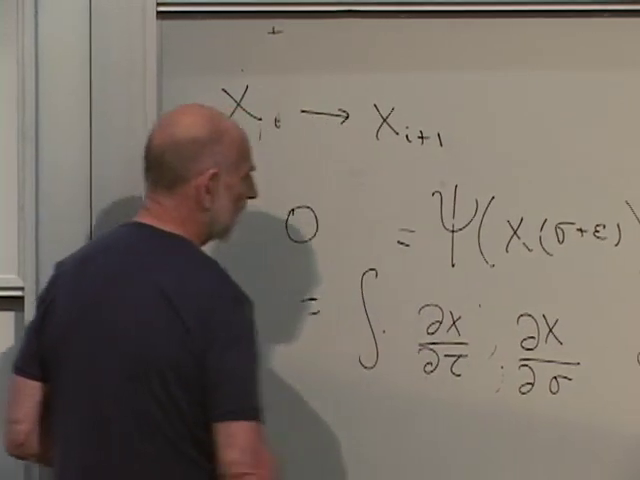
\includegraphics[width=0.75\textwidth]{lecture_04_figure_12.png}
  \caption{波動汎関数の微分が運動量と同定された後の積分された生成子。}
  \lectureframe{01:05:10}
  \label{fig:l04-generator-board}
\end{figure}

\subsection{生成子はエネルギー差である}

\eqref{eq:l04-left-right-energies}における二つの表式の和は全エネルギーである。それらの差は
\begin{align}
  E_L-E_R
  &\propto
  \frac12\int_0^{2\pi}d\sigma\sum_I
  \left[
    (\dot X^I+X^{I\prime})^2\right.\nonumber\\[-0.25em]
  &\hspace{7em}\left.
    -(\dot X^I-X^{I\prime})^2
  \right]\\
  &=
  2\int_0^{2\pi}d\sigma\sum_I
  \dot X^I X^{I\prime}.
  \label{eq:l04-energy-difference}
\end{align}
この積分は物理的状態を消滅させなければならない生成子である。したがって
\begin{equation}
  E_L-E_R=0,
  \qquad\text{or}\qquad
  N-\widetilde N=0.
\end{equation}
レベルマッチングとは、\(\sigma\)座標の原点が観測不可能であるという主張である。

\begin{figure}[H]
  \centering
  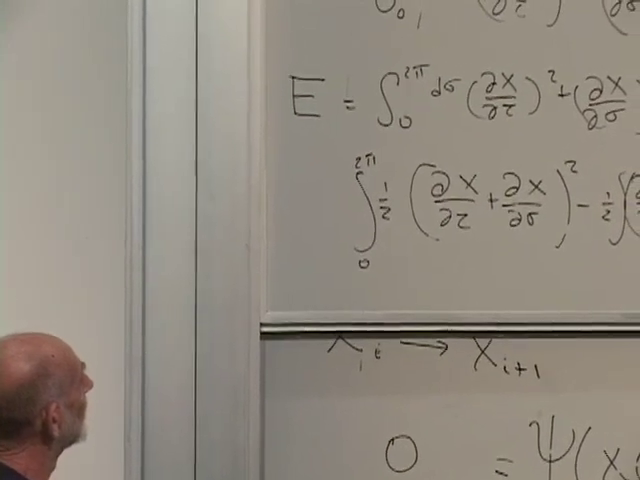
\includegraphics[width=0.78\textwidth]{lecture_04_figure_13.png}
  \caption{レベルマッチングの導出の最後に一緒に表示されたエネルギー和と差。}
  \lectureframe{01:06:40}
  \label{fig:l04-energy-difference-board}
\end{figure}

\begin{classroomqa}
\audiencequestion{なぜ表示された式は1/2の因子を異なる場所に置いているように見えるのか？\lecturetimestamp{01:06:28}}
\lecturerresponse{相対的な構造のみが使われている。一貫した全体的規格化を復元すると、完全平方の恒等式\eqref{eq:l04-energy-square-completion}における1/2が得られる。和は全エネルギーを与え、差は\(\int d\sigma\,\dot X X'\)に比例したままである。その消滅、したがってレベルマッチングは、その共通の規約に依存しない。}
\end{classroomqa}

この拘束条件は素朴な振動子スペクトルの大部分を取り除き、まともな粒子多重項を形成できなかった状態をまさに取り除く。開弦の光子は取り除かない。開弦はこの閉ループ条件に従う二つの独立な循環セクターを持たないからである。閉弦に対しては、重力子、ディラトン、反対称テンソルまたはアクシオン的状態、およびより高次のマッチしたレベルを残す。
\editorialnote{共変な弦の量子化では、レベルマッチングはゼロモード条件\(L_0-\widetilde L_0=0\)であり、世界面拘束系の一員である。ここでの導出は、閉弦の周りの並進に対する不変性として、その直観的起源を分離する。}

\section{左右の二つの意味}

ここで「左右」という言葉には二つの無関係な用法がある：
\begin{enumerate}
  \item \(X_R(\tau-\sigma)\)と\(X_L(\tau+\sigma)\)は、内在的な\(\sigma\)円に沿った反対方向への伝播を記述する。
  \item \(c_+^\dagger\)と\(c_-^\dagger\)は、物理的な横断\(xy\)面における円偏光を記述する。
\end{enumerate}
レベルマッチした重力子状態は、各世界面方向から一つの振動子を含む。それら二つの振動子はそれでも同じ時空ヘリシティを持ち、\(h=+2\)または\(h=-2\)を生じうる。これら二種類の左右を混同すると、スペクトルは矛盾しているように見えるが、実際はそうではない。

\section{「基本的」とは何を意味するか？}

開弦と閉弦がこの初等的なレベルで量子化された後、自然な疑問が残る：弦は最終的な構成要素なのか、それとも弦自身が何か別のものからできているのだろうか？

\begin{classroomqa}
\audiencequestion{弦を最も基本的な対象と見なし、その下に何もより小さなものがないという証拠や理由はあるか？\lecturetimestamp{01:10:44}}
\lecturerresponse{有用なパラメータに依存しない答えはない。ある領域で素粒子的に見える自由度は、別の領域では重く、拡がり、明らかに複合的になりうる。基本的とは、考察中の結合定数においてどの変数が有用な記述を与えるかについての主張として読むのが最善である。}
\end{classroomqa}

電荷と磁荷は、この答えの最も明快な模型を与える。理論が電荷 \(e\) と磁荷 \(g\) を含むとしよう。モノポールに付随する観測不能なディラック弦は
\begin{equation}
  eg=2\pi n,
  \qquad n\in\mathbb Z.
  \label{eq:l04-dirac-quantization}
\end{equation}
を要求する。最小の電荷に対しては \(n=1\) である。ディラック弦の周りを回る荷電粒子は位相 \(e^{ieg}=1\) を獲得するので、補助的な弦は検出できない。

\begin{figure}[H]
  \centering
  \begin{minipage}[t]{0.58\textwidth}
    \centering
    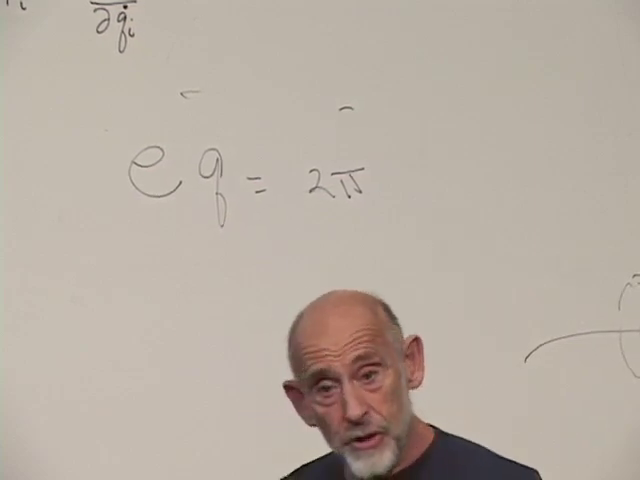
\includegraphics[width=\textwidth]{lecture_04_figure_14.png}
    \par\smallskip\footnotesize (a) 黒板におけるディラック量子化。
  \end{minipage}\hfill
  \begin{minipage}[t]{0.36\textwidth}
    \centering
    \begin{adjustbox}{max width=\linewidth}
    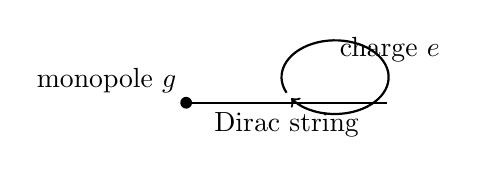
\begin{tikzpicture}[scale=0.85]
      \fill (0,0) circle (2.5pt);
      \node[above left] at (0,0) {monopole \(g\)};
      \draw[thick] (0,0) -- (3.0,0);
      \node[below] at (1.5,0) {Dirac string};
      \draw[->,thick] (1.5,0.15) arc[start angle=205,end angle=-145,
        x radius=0.8,y radius=0.55];
      \node[right] at (2.15,0.8) {charge \(e\)};
    \end{tikzpicture}
    \end{adjustbox}
    \par\smallskip\footnotesize (b) 弦の周りの位相実験。
  \end{minipage}
  \caption{電荷と磁荷はディラック条件によって逆の関係にある。}
  \lectureframe{01:13:20}
  \label{fig:l04-dirac-board}
\end{figure}

\(e\) が小さいなら、電気的変数における通常の摂動論が有用である。追加の電気的頂点を持つファインマン図はますます抑制される。しかし \eqref{eq:l04-dirac-quantization} はそのとき \(g\) を大きくするので、磁気的頂点におけるダイアグラム展開は有用でない。通常の無次元結合定数で表すと、
\begin{equation}
  \alpha_e=\frac{e^2}{4\pi},
  \qquad
  \alpha_m=\frac{g^2}{4\pi},
  \qquad
  \alpha_e\alpha_m=\frac{n^2}{4}.
  \label{eq:l04-dual-couplings}
\end{equation}
弱い電気的結合は強い磁気的結合であり、その逆も成り立つ。

強結合のモノポールもまた、電気的記述から見て複雑に見える。その場のエネルギーは大きく、ゲージ場の揺らぎと仮想的な磁気的荷電対の激しい雲によって着飾られている。それは重く広がった対象として振る舞い、電気的摂動級数にとって出発点として不適切である。これはそれがより根源的でないことを証明するものではない。それは、その領域にとって誤った基本変数であることを述べているのである。

ここで \(e\) を連続的に増加させると想像しよう。量子化条件は \(g\) を減少させることを強制する。自己双対領域の近くではどちらの記述も特に弱くはなく、それを超えると磁気的変数がより単純で軽いものになり得る一方、電気的対象は強く着飾られるようになる。どちらの電荷を基本的と呼ぶべきかは、理論の物理的内容を変えることなく変化したのである。

\subsection{ウィグナーの問い}

この曖昧さはかつて、ヒッグス粒子が基本的か複合的かという議論の中で表面化した。ユージン・ウィグナーは複合的とは何を意味するのかと繰り返し問うた。提案された一つの区別は崩壊であった。おそらく基本的な対象は崩壊できず、複合的な対象は崩壊できるというものである。しかし基底状態の水素原子は崩壊できず、明らかに複合的である。陽子は安定であり得る一方で中性子は崩壊するが、それによって一方が基本的で他方が意図された意味で複合的になるわけではない。あらゆる単純な定義は新たな反例を生み出した。

ヘーラルト・トホーフトは、操作的基準によって議論を終わらせた。すなわち、対象を基本的と考えることが有用であるとき、その対象は基本的である。これは回避ではない。それは、基本的とは力学が単純である変数を同定することを認識しており、単純さは結合定数と環境に依存し得るのである。

\section{M理論へ向けて}

弦理論はこの役割の交換を特に鋭い形で実現する。あるパラメータ領域では、弦は軽く摂動的である一方、Dブレーンは弦の自由度から作られた重いソリトン的複合体のように見える。パラメータが変化すると、Dブレーンはより軽い基本的対象になり得て、最初の領域で弦として記述された配位はそれらの言葉で再解釈され得る。基本的に見えたものが複合的になり得て、複合的に見えたものが基本的になり得る。

古い還元主義的描像は、大きなものからより小さな構成要素へ、そして最終的に唯一の最下層へと向かう一方向の下降を示唆する。双対性はより線形でない何かを示唆する。すなわち、結合定数が変化するにつれて記述は互いに変換し得て、どこでも特権的な単一の変数集合は存在しないのである。これが、次の主題であるM理論に接近する視点である。

臨界次元がボソン弦では26、超弦では10である理由という問いは、ここでは未解決のままである。先に進む前にあらゆる技術的問題を解決するよりも、今や視点を変えて、M理論が適切な極限でいかにして弦理論を生み出し得るかを問う。